\chapter{Firm model}
Our treatment of the urban surplus which is central to this thesis, is illustrated in Figure~\ref{fig:Agglomeration-surplus}. In the lower left, we illustrate a single firm with decreasing returns to scale operating at its optimal scale, $n$. The thick diagonal line represents the effect of increasing the number of firms operating at the optimal scale. It is the constant returns (CRS) line. If congestion effects from bringing a large number of firms together were dominant, a city would exhibit decreasing returns to  scale,  $N$, and agglomeration would not occur. Research indicates that cities exhibit increasing returns to scale, illustrated by the upper line, which shows the city generating an increasing surplus as it grows, which is the increasing returns to scale case. The curvature of the line is determined by a function of the form $N^\gamma$, which we include in the production function for urban firms. 

We assume there are many firms operating at their optimal scale in both the rural and urban sector, but the production function of the urban firm is augmented by the term $N^\gamma$. 

NOTE ON EXPONENTS

\begin{figure}[htb]
    \centering

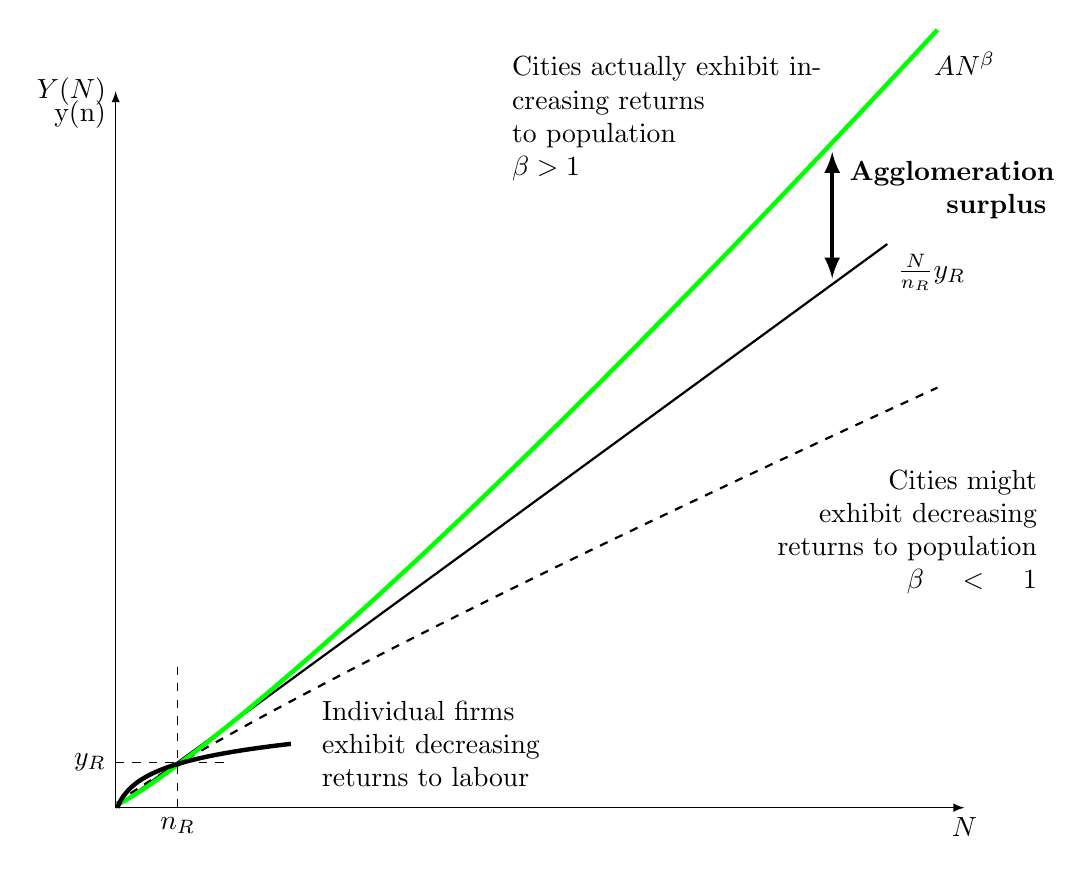
\begin{tikzpicture}[scale=.7, my plot/.style={thick, smooth, samples=100, domain=0.1:2.2},
plot2/.style={thick, smooth, samples=100, domain=0.1:14.99},
                    my grid/.style={dashed,opacity=0.5, every node/.style={black,opacity=1}},
                    my axis/.style={latex-latex}]
 
 \draw[my axis] (0,13)node[left] {$Y(N)$} --(0,0)-- (15.4, 0) node[below] {$N$}; 
%creates the axis 
 \node at (0,13)[below left]{y(n)};
 
\coordinate (origin) at (0,0);
\def\x{0.45}
\def\y{2.1}
\def\b {$15/(2*ln(\y)+.05)$};
%\def\p{0.55} % define the x, y and p )(midpointvalues
%\draw[my plot] (0,0) plot (\x,{ln(\x)});  %Draws curve
%\draw[my plot] (0,0) plot ({\x-.08},{2.3+ln(\x)}); 
\coordinate (Uy) at (\y,{2*ln(\y)+.05});

% THREE SCALE POSSIBILITIES
\draw [thick, ](0,0)--(14, 10.22583)node[below right]{$\frac{N}{n_R}y_R$};   %diagonal line CRS
\draw[plot2, dashed] (0,0) plot ({\x-.08},{(\x)^0.9/1.5 }); %DRS
\draw[plot2, ultra thick, green] (0,0) plot ({\x-.08},{(\x/1.5)^1.15});%
\node at (15.4, 13.5){$AN^\beta$};

%  TEXT
\node at (13.8,12.5) [left, text width=4.5cm]{Cities actually exhibit increasing returns\\ to population\\ $\beta>1$};%IRS
\node at (13.5,5)[text width=4.5cm, align=right] {Cities might\\ exhibit decreasing \\returns to population \\ $\beta<1$};% DRS

% ARROW
\draw[latex-latex, ultra thick] (13, 11.9)--(13, 9.6);
\node at (15.1, 11.2)[ text width=2.5cm, align=right]{\textbf{Agglomeration\\ surplus}};
%\draw[latex-latex] (13, 8.4)--(13, 9.5)node [below right, text width=1.5cm]{\textbf{$\pi$}};

\begin{scope}[ yscale=.75,xscale=1.5]% shift={(1.9,0)} ,
	\coordinate (Uy) at (\y, {2.3+ln(\y)});
  \draw[my plot,ultra thick] (0,0) plot ({\x-.08},{1.15+ln(\x)/2})node[right=.25cm, text width=3.9cm]{Individual firms\\ exhibit decreasing\\ returns to labour}; % production function for generic ferm
	\draw[dashed](.75, 0)node[below]{$n_R$} --(.75, 3.4);
    \draw[dashed](0,  1.1)node[left]{$y_R$} --(1.4,  1.1);
\end{scope}
%
%
%\begin{scope}[shift={(1.9,0)}]
%
% \def\x{0.45}\def\y{2}\def\p{0.55} % define the x, y and p )(midpointvalues
%\draw[my plot] (0,0) plot (\x,{ln(\x)});  %Draws curve
%
%\coordinate (start plot) at (0.6,{ln(0.16)}); % domain start
%\coordinate (end plot) at (10,10); % domain end
%%\draw[my axis] ([shift={(-0.5cm,0.5cm)}]start plot |- end plot) node[left] {$Y(\cdot)$} |- node[coordinate](origin){} ([shift={(0.5cm,-0.5cm)}]start plot -| end plot) node[below] {$L$}; %creates the axis a little 
%
%\coordinate (Ux) at (\x,{ln(\x)}); % set the u(x) coordinate on the curve. Not used
%\coordinate (Uy) at (\y,{ln(\y)}); % set the u(y) coordinate on the curve
%
%\draw [](origin)--(Uy)  ; 
%
%\draw[my grid] (Uy) |- node[below]{$L*$} (origin) |- node[left]{$Y^*$} cycle;%below from on curve, the 
%
%\end{scope}

\end{tikzpicture}

    \caption{While each individual firm exhibits decreasing returns to scale, the city as a whole exhibits increasing returns to scale, and thus produces an agglomeration surplus, $A(N^\beta)-\frac{N}{n}Y_F$.}
    \label{fig:Agglomeration-surplus}
\end{figure}

We need to distinguish the parameters of production functions for rural and urban firms and for the city as a whole. We assume that  rural and  urban firms use the same Cobb-Douglas technology $Y=A_FK^{\alpha_F}L^{\beta_F}$. The difference is that the urban firm enjoy a  multiplicative agglomeration externalize $N^\gamma$ which we assume is negligible for the rural firm and omit. $Y=A_FN^\gamma  K^{\alpha_F}L^{\beta_F}$.

In addition, there is an aggregate production function for the city from the scaling literature which we write $Y=AN^\beta$. We omit the subscript $C$ for city from  the aggregate production function.    



\subsubsection{number of firms} $F_{t}=\frac{N_{t-1}}{n^{target}_{t-1}}$. Firm formation uses current variables to set number of firms for the next period 

\subsubsection{actual urban firms' employment} 
$n_t^{actual}= \frac{N_t}{F_t} $. Available workers are divided among existing firms.   


\textbf{actual urban firms' capital} in period t should be based on planned output rather than the labour available in the period, so we begin with the marginal productivity of labour equation, \[\omega_{t}+\psi = \frac{\beta_{F}Y^{target}_{t-1}}{n_{t-1}^{target}}\]
which gives us 


\textbf{urban firms' actual marginal product of labour}
\[MPL_{t} = \frac{\beta_{F}Y^{actual}_{U,t}}{n_t^{actual}}\] \noindent Firms observe their output, Yt and find  MPL= that they want to set equal to the wage. Al the values have been determined in the previous  and $n^{actual}_t$ is calculated using values from the  previous period, we get

\textbf{urban firms' output} by solving the above for Y
\[Y_{U,t}=  n_t^{actual}\frac{\omega+\psi}{\beta_{F}} \] 
This is used to calculate target employment.
% \item[(urban firms' capital)] (May not be needed)
% \[ K_{U,t}= \frac{\alpha}{\beta} \frac{n_{t-1}(\omega_{t-1}+\phi)}{r}\]


{\color{red}
\subsubsection{urban firms' target employment for $t+1$} Firms examine their own output and marginal product of labour, all calculated with values determined in the previous period. Following the  optimality rule, MPL=wage and MPK-r, they compute a target value for $n$ and $K$
\[ n^{target}_{t+1}= \frac{\beta Y_{t}}{\omega_t + \phi} \]



\subsubsection{aggregate urban labour demand of existing firms $N_{F,t+1}^{target}$} 

\[N_{F,t+1}^{target} = \frac{n^{target}_{t+1}}{n^{actual}_{t}} N_t\].   
This makes sense because Y is produced with the previous year's target assuming  $\gamma$ was constant but  $\gamma$ could have risen. (This should be the same result as  multiplying $n^{target}_{t+1} \times F_{t} $)



\subsubsection{New entrant labour demand,  $n\Delta F$} Firms enter when $MPL > wage$, which with existing technology permits profit making. New firms would set the same target employment as existing firms. 
\[n\Delta F =Z\frac{MPL_t-\omega_t -\psi}{\omega_t +\psi}F n^{target}_{t+1}\]
This makes sense because the number of entrants as a fraction of the existing number of entrants should be larger when the profit margin is larger. New firms would set the same target employment as existing firms and 

\subsubsection{Aggregate urban labour demand of existing firms $N_{Total,t+1}^{target}$} 
\[N_{Total,t+1}^{target}= N_{F,t+1}^{target}+n\Delta F\]

\subsubsection{Number of firm adjustment} 
\[F_{t+1}=\frac{N_{Total,t+1}^{target}}{n^{target}_{F,t+1}}\] 
This adjusts over time, keeping the firm labour force near the optimal level. 
{
\color{blue}
    \subsubsection{Wage adjustment for NEW workers} 
Firms want to increase output so they bid for new workers
\[wage_t^{new}= (1-adj_\omega)\omega_{t-1} + adj_\omega MPL_{t-1}  +\psi\] 

\subsubsection{Wage adjustment for EXISTING workers }
Existing workers demand catchup increases
\[ wage_t^{existing}= (1-adj_{exist})*\omega_{t-2} + adj_{exist}* wage_{t-1}^{new}  +\psi\]
Do we have to worry about workers switching firms? Would switchers get the full  bid new workers get? 
}
}
\textbf{wage adjustment factor} This is the fraction by which desired labour exceeds actual labour
\[\nu_t =\frac{N^{target}_{t+1}-N_{t}}{N_{t}}\]
or 
\[\nu_t =\frac{n^{target}_{t+1}-n_{t}}{n_{t}}\]



\subsubsection{Wage adjustment} 

\textbf{Wage calculation}
Firms make one decision faced with a market wage. They choose a target workforce. This is typical in \glspl{competitive market} where firms are price-takers. 


When \textbf{aggregate} firm labour demand exceeds N, wages rise at the city level

To get labour supply $N^s$ in terms of  $\omega$ we combine $N=f^2 *density$ and $f=2\omega/c$. 

So $\die{N^s}{omega}=4fden/c$ and \[\Delta \omega=  \frac{c}{4fden}\Delta N = \frac{c}{4fden}(N_{Total,t+1}^{target}-N_t)\]
This is the discrete wage adjustment that would attract the desired number of new workers, providing housing is available.\footnote{What happens is housing is not available? Maybe workers can't come to the city until the housing stock adjusts. Firms have labour shortages.  The wage stays high or may rise more. House prices will rise.} We can think of this as the wage demand of new workers.\footnote{What if only new workers get the new wage? This is interesting: firms will make excess profits. New firms will be attracted by excess profits but may not be able to get workers at the old wage!}

Should the adjustment occur in a single period?

It may be useful to put in an adjustment factor $adj \le 1$.
\[\omega_{t+1}=\omega_{t} + adj \Delta_t  \omega\]




% Common to think of the variations in local wages as variations around a mean, in this context - perfect labour market.
% We're using this number at the aggregate level, raise the market wage to a level that attracts that many. Divide available workers among the firms, then they want to raise the wage again. It's more transparent to do it at the aggregate level than at the firm level, but we still have the rising supply curve. A more detailed agent model could implement the hiring and wage adjustment mechanisms for firms directly, but the side effect of increased complication is it also can obscure the clarity of the rent results, our focus with this work. 



\section{Firm initial values}

\subsubsection{Firm $Y_{F,i}=A_FK_i^\alpha n_i^{\beta_F}$}
We use the familiar Cobb-Douglas production function \cite{chiangFundamentalMethodsMathematical2002} to set relationships among variables that are consistent with basic neoclassical production theory. 
\begin{description}

\item[initial urban wage premium] = $\omega_0 = (wage\_premium\_ratio) * \psi = p*\psi $

\item[initial labour force for urban firms] $n_0=n_R$.  Initially we will try values similar to the rural firm size and vary it  %*****%may have implica=tions later for the notation

\item[Initial wage premium] $\omega_0=p_0*\phi$

\item[Initial wage] = $\omega_0=\omega_t +\psi =(1+p_0)\psi)$
%The wage  is set as the marginal product of labour for initialization of the model. 

\item[labour cost for typical rural firm] $L_R = n_R*\psi$. This is expressed as a money quantity: e.g., 100 workers * \$40,000/worker.  

% \item[Initial labour cost for typical urban firm] ]  $L_U = n_R(\psi+\omega_0)$.

\item[output for typical rural firm]  
\[Y_R=\frac{n_R*\psi}{\beta_F}\]
This is a constant for any initial values. Derived from the marginal productivity condition. See item~\ref{item-paramlist-firm-level} in the orange  block. The numerical calculation is done  for a firm with 100 workers and a marginal product of labour of $\psi$. I get \$20 million for those values. 


\item[initial output for an urban firm] 
\[Y_0^U=N_0^\gamma Y^R\]  
Taking the marginal product with respect to $n$, we get a useful fact that will allow us to tie down $\gamma$
\[Y_{U,0}=\frac{n*(\psi+\omega)}{\beta_F}\]

\item[capital for typical rural firm] (Derived from the marginal productivity condition.)
\[K_R=  \frac{\alpha_R Y_R }{r}\]
This is also a constant.
 
\item[initial capital for an urban firm] (Derived from the marginal productivity condition.)
\[K_{U,0}=  \frac{\alpha Y_{U,0} }{r}\]
This is also a constant.

\item[scale factor A for typical  firm] 
\[A_F= \frac{Y_R}{K_R^{\alpha} {n\psi}^{\beta_F}}\]
We will assume that this is a constant used for both rural and urban production functions. (The explicit function is a bit  messy but the numeric value is easily computed because we have $L_r=n_R\psi$, and have calculated $Y_F$, and  $K_F$). The prefactor.

\end{description}
% \textbf{NOTE: With the initial values calculated in this section $\omega$ is consistent with $N_0$.as a result, population should not grow.}

\begin{quotation} \color{orange}
\section{Firm level production}   
(This is incorporated above.) We want the marginal product of labour in the rural economy at the firm level to be at least close to \$40,000.  We can create a generic rural firm and then consider an urban firm with agglomeration effects to get the parameters we need. 

Firm employment $L$ is small relative to  urban employment {N}. Assume it is 100 workers. 

Assume that the rural production function is 
\[ Y_{iF}^R=A_{F} K^{\alpha_F} L_F^{\beta_F} \]
where  $L_F=n*\psi$, $\alpha_F=0.18 $,  and $\beta_F=0.76$.notice that the MPL is the partial derivative with respect to $n$ and not L. 
\footnote{These values give us diminishing marginal product at the firm level. If we require product exhaustion we have factor shares of  0.8 and 0.2.The tricky point is that factor share are 
 $\frac{\alpha}{\alpha + \beta}$ and $\frac{\beta}{\alpha + \beta}$
(*If not there is surplus profit  which we will ignore.)}   
The marginal products pf labour and capital are 
\[MPL=n*\beta_F Y_F/L_F=\$40,000\] and\[\ MPK=\alpha_F Y_F/K_F =0.05\]
From the first, 

\[Y_F=\frac{n*\psi}{\beta_F}=\frac{100*\$40,000}{0.72}=\$5,555,556\]
This is firm revenue. From the MPK, 

\[K_F=  \frac{\alpha_F Y_F }{r}=\frac{0.18 *\$5.5555\ million}{0.05} =\$20\ million = 1.039568 \]

We now have the capital, labour and output for a model firm with a marginal product of labour  equal to the subsistence wage we have chosen. We can calculate the \textbf{scale factor} 

\begin{equation}  
A_F= \frac{Y_F}{K^{\alpha_F} L^{\beta_F}}=\frac{5,555,000}{20,000,000^{\alpha_F} 100^{\beta_F}} = 1.039568 \label{eqn-AR}\end{equation} 
So $A_F$ can be computed using equation~\ref{eqn-AR} for any set of coefficients and firm size. Expanding the expression,

% \begin{equation}  %   arithmetic error here
% A_F 
% =\frac{\frac{n*\psi}{\beta_F}}{\frac{\alpha_F  \left(\frac{n*\psi}{\beta_F} \right)}{r}  L^{\beta_F}} 
% =\frac{\frac{n*\psi}{\beta_F}}{\frac{\alpha_F \frac{n*\psi}{\beta_F} }{r}  L^{\beta_F}} 
% =\frac{r}{\alpha_F  L^{\beta_F} }
% =6.944444e-08???? \label{eqn-AR2}\end{equation} 

Furthermore, we can compute the output for a city of size N if it consists of $N/n$ firms of this type. With a population of 10,000, for example,  there would have to be  100 firms and an output of \$555,555,600. 

 \subsubsection{The urban level of production}
 \textbf{This section now redundant and has been commented out}
% We now consider that this firm operates in the city and enjoys  urban agglomeration benefits. The value of the  marginal product of labour must rise to $\psi+\omega$. We to know  the urban wage premium that is consistent with the subsistence wage. Papageorgiou \cite{papageorgiouOccupationalMatchingCities2022} found a 4.1\% premium. D'costa and Overman   show that working in London is associated with a 35.5\% higher wage than working in a rural area. The comparable figures are
% 10.6\% for big cities and 8.3\% for small cities and an elasticity of wages with respect to city size of 1.6\%.. Estimates of the premium are lower  when they control of individual characteristics.   

% If the $ scale\ coefficient=1.12$, $=\omega$ would be $1.12*\psi$, or $4,800$. 

% This supports an urban wage premium of $\omega\$8,000$.

% We need to have a population size or a number of firms with a firm size. Assume the population is 10,000 and firms still have 100 workers. (All firms will have the same marginal product of labour in a competitive labour market, so size should not matter.)

% \[Y^U=A^R N^\gamma K^\alpha L^\beta = N^\gamma Y^R\]
% where $N^\gamma$ represents the agglomeration effect. The marginal product of labour is 
% \[MPL^u=\$44,800=N^\gamma \beta Y^R/L=N^\gamma *\$40,000\]
% so $N^\gamma= 1.2$ and $\gamma = \frac{log(1.12)}{log(10,000)} =.012$. 


% This value is consistent with an empirical  value for  the agglomeration exponent of $\beta =  1.012$. The value is much lower than empirical estimates. Furthermore, if we consider the same firm structure and a population of one , the value falls, which suggests that agglomeration effects are not scale-independent, but instead increase with urban size. $\beta$ may itself be a function of $N$.

% % A second interesting possible implication of our calculation is that only part of the agglomeration effect appears in wages. Urban rents  are large, but agglomeration effects are much larger.
\end{quotation}



\footnote{Tørsløv et al \cite{torslovMissingProfitsNations2023} show that affiliates of foreign multinational firms are an order of magnitude more profitable than local firms in a number of low-tax countries. Leveraging this differential profitability, they estimate that 36\% of multinational profits are shifted to tax havens globally. US multinationals shift twice as much profit as other multinationals relative to the size of their foreign earnings.}


\textbf{appendix-05-agglomeration-model - REDUNDANT} %\renewcommand{\sfdefault}{phv}

\section{Initial values for  the agglomeration parameter}
A segment is now redundant and has been commented out

\vspace{5lines}

% {\Large  $Prefactor = 1506.712$ based on width=height=10 and density=100} and agglomeration\_coefficient= 1.2,
% We need to get the scales of the parameters and the population size roughly consistent.

% I assume the 10X10 grid is full. 

% \section{Computing the prefactor: details}
% We have set the subsistence\_wage to \$40,000.

% The urban wage premium is in the range of 13-20\%  Assume 20\% and we get \$8,000

% Under the neoclassical assumption  \$40,000 is the  marginal productivity of rural worker

% The urban production function is 
% \[Y=AN^\beta\]
% \[Y=prefactor*working\_population**scaling\_exponent\]

% where $working\_population = width*height*density$ 

% so 
% \[Y=prefactorA*(width*height*density)^{\beta}\]

% We have more conditions that this has to satisfy: The marginal product must be consistent with the urban wage and the distribution rule. The wage cannot add up to more than total output output. Workers cannot get 1.2Y/N, for example. With CRS they would get 0.8Y/N.    

% \subsection{approach one: from agglomeration surplus}
% \[urban\_wage= subsistence\_wage + wage\_share * agglomeration\_surlpus\]
% The \textbf{agglomeration surplus} is the excess relative to the CRS case when $\beta=1$:
% \[agglomeration\_surplus= A(N^{1.2} -N^1) \]
% The urban wage premium is then the share for each worker:
% \[\omega= wage\_share * \frac{agglomeration\_surlpus}{N}\]

% and this becomes
% \[\omega= wage\_share * A\left(\frac{N^{1.2}-N^1}{N}\right)=1 * A\left(N^{0.2}-1\right)\]

% To see what this looks like, consider a population of 10,000 when  wage\_share=1
% \[\omega= \$8,000 = A\left( 6.309-1 \right)\]

% {\Large So $A = 1506.712$ based on width=height=10 and density=100}  

% Smaller N makes A bigger

% % Say width=height=15 and density= 200:
% % \[\omega= \$8,000 = A\left(10000-1\right)\]

% \subsection{Approach 2: from Marginal product and subsistance wage}
% % We want the marginal product of labour in the rural economy at the firm level to be at least close to \$40,000.

% % Firm employment $L$ is small relative to  urban employment {N}.  We can create a generic rural firm and then consider an urban firm with agglomeration effects to get the parameters we need. 

% % Assume that the rural p[rooduction function is 
% % \[Y^R=A^R K^\alpha L^\beta\]
% % where $\alpha=0.2$  and $\beta=0.8$. The marginal products are 
% % \[MPL=\beta Y/L=\$40,000\] and\[\ MPK=\alpha Y/K =0.05\]
% % From the first, 

% % \[Y=\frac{L*\$40,000}{0.8}=\$5\ million\]

% % This is firm revenue. From the MPK, 

% % \[ \frac{0.2 \$5\ million}{0.05}=K =\$20\ million \]

% % We now have the capital, labour and output for a model firm with a marginal product of labour  equal to the subsistence wage we have chosen.

% % We now consider that this firm operates in the city and enjoys  urban agglomeration benefits.  If the scale coefficient=1.12$,$ $\omega$ would be as a first appr Say that the marginal product rises to \$48,000. This supports an urban wage premium of $\omega\$8,000$.

% % We need to have a population size or a number of firms with a firm size. Assume the population is 10,000 and firms have 100 workers. All firms will have the same marginal product of labour in a competitive labour market, so size should not matter. 

% % \[Y^U=A^R N^\gamma K^\alpha L^\beta = N^\gamma Y^R\]
% % with a marginal product of 
% % \[MPL^u=\$48,000=N^\gamma \beta Y^R/L=N^\gamma *\$40,000\]
% % so $N^\gamma=1.2$ and $\gamma = .019$. 


% This value is consistent with an empirical  value for $\beta$   1.02. The value is lower than empirical estimates. Furthermore, if we consider the same firm structure and a population of one million the value falls, which suggests that agglomeration effects are not scale-independent, but instead increase with urban size. $\beta$ may itself be a function of $N$.

% A second interesting possible implication of our calculation is that only part of the agglomeration effect appears in wages. Urban rents  are large, but agglomeration effects are much larger.


 

% %\[subsistance_wage= MPL(\beta=.= \]
 % bbbb{appendix-05-agglomeration model}



\begin{enumerate}
\item To start with a population of around 10,000, we begin with width = 10, height = 10 and \textbf{density} per unit of 100. 

\item If we arbitrarily assume an initial wage premium around 20\%, and wish to start near equilibrium, % bettencourt assumed aggomeration exponent is indepent)
we can select transportation costs. A transportation cost of 0.1  would give a distance of $\omega/.01$, which is huge. Could this be 1/10 of the starting wage premium $\omega_0$? It would then be \$800 per year, per unit distance and would give us height and width of 10. 
% (divide into omega) - we want to start close to equilibirum. omega/cost = width
\item We should have a wage premium of about \$8000 to be consistent with the subsistance wage. % since we are assuming the wage premium of around 20%. Total wage has to be subsistence wage + wage premium, think of an average rural subistance wage seems like 45K .. 

\item Your proposed prefactor was 0.2,  251. It should be very large, based on the above numbers and the consistency constraints. I get 1507 in appendix-05-agglomeration model

\item Teminology: Y=prefactor*N**scaling\_exponent

\end{enumerate}

\begin{lstlisting}
def __init__(self, width = 50, height = 1,  # ****
             transport_cost_per_dist  = 0.1,    # c   ****
             subsistence_wage         = 40000. # psi
             working_periods          = 20,     # in years ****
             savings_rate             = 0.2, ****
            #  initial_savings: if agents save anything before reaching working age
             init_wage_offer          = 10.,  #. Makes no sense  ****
             init_interest_rate       = 0.05,

             #AGGLOMERATION MODEL features  -20% wage premium over subsistence wage, Y=prefactor*N**scaling exponent
             prefactor                = 0.2, # 251., ??????  ****. should be very large. I get 1507 
             # Prefactor - should be much higher than YES scaling_factor           =   # this is A scaling_exponent         =  1.13 # this is beta in LOBO. ****
             agglomeration_ratio      = 1.2,  # beta, was 
             wage_share               = 1.0,  # of agglomer3ation benefits
             workers_share            = 0.8   # emponent? in Slae models?
             property_tax_annually    = 0.04, # tau, was c
             mortgage_period          = 5.0,  # T, in years
             housing_services_share   = 0.3,  # a
             maintenance_share        = 0.2,  # b
             r_prime                  = 0.05,
             r_premium                = 0.005, ****
            #  r_premium_bank = 0.00, # TODO: heterogenous discount rates and premiums
             ):
\end{lstlisting}

\subsection{Workers share}
The worker's of the surplus, $lambda$ It might be 0.8. It is used in...

NOTE: 0.8 is the value of beta in a Cobb-Douglas, corresponding to the wage-share in production. It is the value used in Lobo et al



\chapter{Market and bargaining model}


\section{Maximum bids and reservation price for investors }.\footnote{transaction costs on the sale are omitted. Add a parameter or variable.}
There are two types of investment buyers: institutional buyers and homeowners buying an investment home. They use the same investment formula

We assume that institutional borrowers have no limit on their borrowing capacity ($m_i=1$). home. Existing owners face mortgage constraints form Equation ~\ref{eqn-max-mortgage2} and have different rates $r_i^{target},\ \delta_i$, and $r_i$.

Equation~\ref{eqn-property-investment-return1} gave us the rate of return for a property, rented out. An investor will invest if the expected return on their investment is greater than their target rate of return, % that the investor can price offer for the property and still satisfy
defined by the inequality~\ref{eqn-property-investment-return2}, and equation~\ref{eqn-bid-price}, repeated below, gives the maximum bid price:

\begin{eqnarray}\label{eqn-max-investment-bid}
P_{bank}^{max\_bid} & = \frac{\mathcal{R}_N}{(1-m)r^{target}-\delta \left(1 + \dot P_M^e - (1+r)m\right)} 
\end{eqnarray}
This implies for the bargaining process that if any other potential  has  higher maximum bid, an investor can be eliminated. Combine this observation that each potential bidder will bid up to their maximum bid price, and we know that only the two highest bids matter need be considered.  



\subsubsection{Maximum bid second house buyer}

We assume that existing owners with sufficient savings can bid. They are limited by the limits  that the bank imposes  borrowing capacity.   Purchasing a revenue house is only attractive if the rate return on a rental house exceeds the cost of capital $r_i$. Call this the \textbf{profitability constraint} The maximum bid for this investor is given by Equation~\ref{eqn-max-investment-bid} using one period values for $r_i^{target},\ m_i,\ \delta_i$, and $r_i$.

 \begin{eqnarray}\label{eqn-max-second-bid}
P_{second}^{max\_bid} & = \frac{\mathcal{R}_N}{(1-m_i^{max\_permitted})r_i^{target}-\delta_i \left(1 + \dot P_M^e - (1+r_i)m_i^{max\_permitted}\right)} 
\end{eqnarray}
Notice that this simplifies if any of $r_i^{target},\ \delta_i$, and $r_i$ are set equal. It is possible the cost of capital and the target rate will be the same.

Combining the investment \textbf{profitability constraint} and mortgage constraints

\begin{eqnarray}
P_{second}^{max\_bid} & = min \left\{P_{second}^{max\_bid},\ \frac{\mathrm{savings}_i}{1-m_i^{max\_permitted}},\ \mathrm{saving}s_i + M_i^{max\_permitted}  \right\}  \nonumber
\end{eqnarray}

\subsubsection{Reservation prices for investment owners}
If the current owner of an investment  property gets an high offer higher than their own maximum bid, they will always sell.  


\section{New buyer maximum bids and reservation prices }
A new buyer chooses to move if the income in the city, including the wage amenities exceed the rural income after housing costs, $\psi+A^{Rural}$. 

There are two cases - moving as a buyer and moving as a renter.

\subsection{Moving as a renter}
The gain for a potential renter is 
\begin{align}
gain^{rent}=&net^{city}-net^{Rural}\nonumber\\
=&\left[\psi+\omega-cd+\mathbb{A}^{city}-\mathcal{R}\right]-\left[\psi+\mathbb{A}^{Rural}-a\psi\right] \nonumber\\
=&\ \omega-cd+\mathbb{A}^{net}-\mathcal{R}
\label{eq-move-to-rent}
\end{align}
If rent $\mathcal{R}$ exactly capture housing cost and locational rent, the gain reduces to $\mathbb{A}^{city}-\mathbb{A}^{Rural}$. Normally we would expect property rents to capture this component  as well. 

\subsection{Moving as a buyer}
The gain for a buyer is 
\begin{align}
gain^{buy}=&\ net^{city}-net^{Rural}\nonumber\\
=&\left[\psi+\omega-cd+\mathbb{A}^{city}+(\dot p-r_im_i)P-a\psi\right]-\left[\psi+\mathbb{A}^{Rural}-a\psi\right] \nonumber\\
=&\ \omega-cd+\mathbb{A}^{net}+(\dot p-r_im_i)P  \label{eq-move-to-buy}
\end{align}
This requires that the sum of  locational rent, net amenity and net capital gain be greater than or equal to zero for the in-migrant to buy.

The two decisions  are 
\begin{enumerate}
    \item Move only if $max\{gain^{buy},\ gain^{rent}\} \ge 0$, otherwise do not move to the city.
    
    \item Buy a house if $(\dot p-r_im_i)P\ge  \mathcal{R}$, otherwise rent.
\end{enumerate}

The buyer is subject to the mortgage constraints in Equation~\ref{eqn-max-mortgage-combined}.

We will assume that a first-home buyer always takes the maximum mortgage available to maximize the financial return on the transaction. 

The maximum price a new buyer can bid is also given the bank imposed liquidity constraint is given by Equation~\ref{eqn-max-mortgage-combined}, which we repeat here


\begin{align}
P_i^{max\ bid}= min \left\{\frac{\mathrm{savings}_i}{1-m_i^{max\_permitted}},\  M_i^{max\_permitted} + \mathrm{saving}s_i  \right\}   \nonumber  
\end{align}


\subsection{reservation price for retirees}
Both owners and tenants retire. Homes only become available if they move to the country. 



\subsubsection{Why would a renter move to the country?} 
f the rent is greater than the cost of housing in the country and the lost amenity
\[\mathcal{R} > \ a\psi+ \mathbb{A}^{net}0\]


\subsubsection{Why would an owner move to the country?}
Why would an owner sell a home and move to the country? It would be economically advantageous if the interest on income from the sale exceeds the cost of housing in the country and the lost amenity.
\[r_i(P^{realized}-M) >\ a\psi+ \mathbb{A}^{net}\label{eq:movers-gainA}\]


This value provides a \textbf{reservation price}: 
\[P^{reservation} =\ \frac{a\psi+ \mathbb{A}^{net}}{r_i}+M \label{eq:movers-gainB}\]
This just says that the lowest prices one would sensibly accept is the cost of a house in the country plus enough to cover the mortgage, plus capitalized net amenity.\footnote{transaction costs on the sale are omitted. Add a parameter or variable.}

Should a retiree rent the house out? only if the rent exceeds the  interest on income from the sale:
\[\mathcal{R}^{net}>r_i(P^{realized}-M)\]
This value provides a \textbf{another reservation price}: 
\[P^{reservation} =\ \frac{\mathcal{R}^{net}}{r_i}+M \label{eq:movers-gainC}\]


Sellers should use the investment rule calculated before  do determine a  reservation price in the bargaining process. If they can't get a higher price they  can keep the home as a rental  investment and use the home as collateral for a mortgage on a house in the country.
% For a homeowner, the reservation price is tricky. 
% At this point we only have retirement as a hard boundary to consider. That means that the householder wants to sell in the current period. The gain from moving to the country is 
% \begin{equation}
% Gain=P_{ij}^{expected}-M-\frac{a\psi}{r\_prime} - transaction\ costs - Urban Amenity\  
% \end{equation}\label{eq:movers-gain}
% In the initial model  there are no urban amenities and no transaction costs. We could subtract an urban amenity term, $U_{ij}$ and an transaction cost from equation~\ref{eq:movers-gain}. The amenity term is likely to have little effect, since a buyer will pay extra for the amenity. the transaction cost is actually large and is likely to significantly affect land allocation efficiency.  

The reservation price in in Equation~\ref {eq:movers-gain} is the minimum provides an incentive to sell a home immediately on retiring from the workforce. 



If the sale is delayed by one period, however, the gain is deferred, so the present discounted cost of waiting is, $Gain*\frac{\delta}{1+\delta}$.\footnote{This is simply (1 minus the discount factor) times the deferred amount.} A seller would accept a lower price to avoid this cost of waiting. 

My suggestion is that $\frac{\delta}{1+\delta}P_{ij}^{expected}$ is the \textbf{initial reservation price} for a homeowner on retirement. If the seller does not get this she reduces the reservation price for the next period by (say) 5\% .


\subsubsection{for the Investor-owner}
\textbf{For financial sector in general including those holding investment properties} the problem is easier if anyone offers more than your maximum bid, you should sell the property. 
\begin{eqnarray}
P_{bank}^{reservation} & =    \frac{\mathcal{R}_N}{(1-m)r^{target}-\delta \left(1 + \dot P_M^e - (1+r)m\right)} \label{eqn-res-price-B} \end{eqnarray}

% P_B & \le    \frac{\mathcal{R}_N}{(1-m)r^{target}-\left[ \delta(1+L(P)- (1+r)m\right]}
We call this  $i's$ maximum bid and compute it for all potential buyers and sellers. In each sale the highest $P_B$ will make the purchase. The denominator can be seen as an adjusted rate of return for capitalizing net rents, analogous to the value of $r$ in  the standard capitalization formula. 



\subsubsection{expected price}
So what is the \textbf{expected price}? this should be the expected price from a weighted price regression.\footnote{Wheaton \cite{wheatonVacancySearchPrices1990} suggests ``The combination of price and expected sales time determines the ``expected price'' for a house: market price discounted by expected sales time.'' In his model, vacancy, matching, sales time, and prices with positive vacancy, matching, sales time, and prices are all jointly determined.} Crudely it might be
\[P_{d,t}^e=\beta_1 d + \beta_2 P_{d,t-1} +\epsilon\]
where $\beta_1$ captures spatial correlation and $\beta_2$ captures serial correlation. In this model $\beta_2=1+\dot P$. This simple relationship would tend to change in each period, so the regression would be repeated  at the end of each period  to be used by everyone in the next period. 

You could add $+ \beta_3 (P_{d,t-1}-P_{d,t-2})$ to capture the changing  price change. 



%\textbf{Alternative approaches to the reservation price}

%\begin{eqnarray}
% P_{person}^{reservation} & =   \frac{\mathcal{R}_N}{(1-m)r^{target}-\delta \left(1 + \dot P_M^e - (1+r)m\right)} \label{eqn-res-price-P} \end{eqnarray}


% \begin{tabular}{p{1.5cm}|p{4.5cm}|p{4.5cm}}
%     & reservation & maximum bid\\\hline
% person-buyer    &   & $min \left\{\frac{\mathrm{savings}_i}{1-m_i^{max\_permitted}},\ \mathrm{saving}s_i + M_i^{max\_permitted}  \right\} $ \\\hline
%    person-new  &   & $min \left\{\frac{\mathrm{savings}_i}{1-m_i^{max\_permitted}},\ \mathrm{saving}s_i + M_i^{max\_permitted}  \right\} $ \\\hline
% Bank    &$ min \left\{\frac{\mathrm{savings}_i}{1-m_i^{max\_permitted}},$$\newline$$\mathrm{saving}s_i + M_i^{max\_permitted}  \right\}  $ & \hline
% \end{tabular}

% ALTERNATIVE, NOT USED CALCULATION
%An alternative way to do this, based on old calculations is to compute the realized mortgage share. The realized mortgage $m_i$

%$m_i$ is follows the wealth based rule, $m_i*$ follows the savings based mortgage rule. The realized mortgage share is whichever of these is chosen by the rule in Equation~\ref{eqn-max-mortgage}.

%$m_i^*$, and get the savings.
% We use $m_i$ in calculating the maximum bid for individuals.
%The \textbf{maximum bid} (price that will be offered) is the minimum of $M^{max_i} +S$ and the maximum bid calculated using $m_i$, , (which is calculated independently) if price
% $P\le \frac{M_i^{max}}{m_i}$ 
% and $m_i^*$ if 
% $P\ge \frac{M_i^{max}}{m_i}$, where 
% \[m_i^*=\frac{M_i^{max}}{P}\]

\subsection{Price setting}
\textbf{We have a many-to-many matching problem}. Many buyers and sellers single sellers for each unit. Therefore, for each property that comes on the market each potential seller has a reservation price $P_{ij}^{reservation}$ and there will be a set\footnote{We could allow potential buyers  to approach potential sellers who have not listed with an offer and allow worker-owners to consider retiring early or becoming tenants if an offer is attractive.  This is only likely if speculative pressures are strong. It may require having multiple institutional buyers to make offers more competitive. In that case, initial offers will be closer to the maximum bid price, tending to pull prices up and benefit potential sellers.}  of potential buyers with maximum bids $P_{ij}^{maxbid}$.


This will appear in your data as a set of bids and a reservation price for each property on the market that must be converted to a price for that property using the bargaining rule. The rule is simple: 
\begin{enumerate}
    \item if there is only one maximum bid above the reservation price, split the difference.

    \item If there are two or more maximum bids above the reservation price, the property goes to the highest  and the price is the second highest
\end{enumerate}

\subsubsection{The process}
\begin{enumerate}
\item \textbf{identify the pool of sellers} for each cycle.
    \begin{enumerate}
        \item Agents who a) own and b) age out
        \item Agent  who failed to sell in the previous period.
        \item the bank
    \end{enumerate}
\item \textbf{identify the pool of buyers} 
    \begin{enumerate}
         \item newcomers, 
         \item individuals as investors.
         \item the bank may buy many, (There must be a capital (C) constraint something like $C/\bar P$ to select a number of bank bids in any period.)
    \end{enumerate}

\item \textbf{count buyers and sellers} and use the counts to identify sellers or buyers' market. \# Sellers > \# buyers is a buyers/ market. For a buyer's market  choose the lower price. \footnote{.The is often done with buyers/vacancies. Changes in this ratio are observed to trigger significant movement in rent r market prices.\cite{wheatonVacancySearchPrices1990}. Lisi and Iacobini \cite{lisiEstimatingHousingPrice2015} found  that in the Italian market, ``the difference between the actual selling price and the price obtained in an ideal situation of frictionless housing market – is remarkable. ... the higher the trading frictions on the demand side (more buyers and less sellers), the higher the actual selling price (the price adjustment is positive), whereas the higher the trading frictions on the supply side (less buyers and more sellers), the lower the actual selling price (the price adjustment is negative). '' (they point out that ``Trading frictions are obvious in the housing market, as it takes weeks or months to buy or sell a house (Caplin and Leahy, 2011; Rocheteau and Weill, 2011).'')}  

%a key role is played by the so-called “time-on-the-market (TOM)”. The time it takes to sell a property or “the expected time until the asset is sold when following the optimal policy” (Lippman and McCall, 1986) – commonly known as the TOM – measures the degree of illiquidity of the real estate asset and is a fundamental characteristic differentiating real estate from financial assets. \cite{lisiSearchMatchingProcess2019}
\item \textbf{The pooling problem}  Houses should go at different prices if they have different net rents.  Assume buyers and sellers are indifferent about location (no  local amenities) so only the net rent matters for the ban and only the full rent for individuals.

\item \textbf{Create lists} for the buyer pool and the seller pool. (The bank can appear on the list many times.) 

If the market is efficient, the allocation will maximize the sum or seller and buyer surplus.

\item To select the set of transactors, \textbf{order the lists}. Buyers from highest to lowest, sellers from lowest to highest.

\end{enumerate}


% Ensure that they are of the same length by dropping the lowest bids or the highest reservation prices. 

\newpage
\textbf{Possibly relevant Example of a matching problem drawn from game theory text}

There are 26  people, some with houses, Each values the house an amount equal to the last three digits of their student numbers. Those on the left of the table don't have a house when the game starts, indicated by a ``0'' in the second column. Those on the right  start with a horse, indicated by a  (1) in the fifth column and half don't. 

\begin{center}
Value and number of houses

\begin{tabular}{|c|c|}
 
\begin{tabular}{lcc}
max bid&start&end  \\ \hline
985  & 0 & 2 \\
829  & 0 & 1 \\
740  & 0 & 1 \\
650  & 0 & 1 \\
643  & 0 & 1 \\
611  & 0 & 1 \\\hline
532  & 0 & \color{red}1  \\
356  & 0 & \color{red} 1   \\
270  & 0 & \color{red} 1  \\
135  & 0 & 0    \\%69 & 1  & 0
   
\end{tabular}

&
\begin{tabular}{lcc}
reservation&start&end \\ \hline
 50 & 1  & 0 \\
127 & 1  & 0 \\
190 & 1  & 0  \\
245 & 1  & 0 \\
 324 & 1  & 0 \\
 522 & 1 & \color{red} 1\\\hline
 738 & 1  &  \color{blue}0 \\
 829 &1  &  \color{blue}0 \\
832 & 1 & \color{blue}0\\
   &  &              \\%69 & 1  & 0 
\end{tabular}

\end{tabular}
\end{center}


 
  \begin{tikzpicture}[scale=.8]
%  \draw [gray, opacity=.7]
 (0,0) grid (7,7);
\draw [<->] (0,10.5) node[above]{value}-- (0,0) -- (10,0) node[below]{Houses};

\draw [red, thick] (0,9.85)node[above right]{985}--(1,9.85)--(1,8.29 )node[above right]{829}--(2,8.29 )--(2,7.40 )node[above right]{740}--(3,7.40 )--(3,6.50 )node[above right]{350}--(4,6.50 )--(4,6.43)node[above right]{643}--(5,6.43)--(5,6.11)node[above right]{611}--(6,6.11)--(6,5.32)node[above right]{532}--(7,5.32)--(7,3.56)node[above right]{356}--(8,3.56)--(8,2.70)node[above right]{270}--(9,2.70)--(9,1.35)node[left]{DEMAND}node[above right]{135}--(10,1.35); 

\draw [blue, thick] (0,.50)node[above right]{50}--(1,.5)--(1,1.27 )node[above right]{127}--(2,1.27 )--(2,1.90 )node[above right]{190}--(3,1.90 )--(3,2.45 )node[above right]{245}--(4,2.45 )--(4,3.24)node[above right]{324}--(5,3.24)--(5,5.22)node[above right]{522}--(6,5.22)--(6,7.38)node[above right]{738}--(7,7.38)--(7,8.29)node[above right]{829}--(8,8.29)--(8,8.32)node[above right]{832}--(9,8.32)node[right]{SUPPLY}; 
%,2.5) ;
%\draw [blue, dashed] (0,4.5) node[left]{large bill}--(8.33, 4.5)-- (8.33,0)node[below] {large user Q};
%\draw [green, dashed] (0,0) --(8.33, 4.5);
%\draw [green, dashed] (0,0) --(1.66, 2.5);

%\draw [<->, shift={(7 cm,0)}] (0,6) -- (0,0) -- (5,0);
\end {tikzpicture}

The gain for any person is the difference between the transaction price  for a house and the amount they value a house




At the same time, for each p. NOT. DONE
\begin{eqnarray}
P_{bank}^{reservation} & \le  P_{person}^{max\_bid} \end{eqnarray}


\begin{lstlisting}
# parameters - max interest payment 
max_mortgage_share = 0.28 # ability to cover a mortgage

# Max mortgage

wealth = property_value - mortgage + savings
mean_weath = sum(wealth)/number_of_people

def get_max_mortgage(self, applicant):
    max_mortgage =  ...
    
    return max_mortgage
\end{lstlisting}





\newpage\hrule
\section{TABLE OF BID AND RESERVATION PRICES}
\hrule




\section{For investors}
 Institutional borrowers have no limit on their borrowing capacity ($m_i=1$). home. Existing owners face mortgage constraints .
maximum bid price:\footnote{transaction costs on the sale are omitted. Add a parameter or variable.}

\begin{eqnarray}\label{eqn-max-investment-bid}
P_{bank}^{max\_bid} & = \frac{\mathcal{R}_N}{(1-m)r^{target}-\delta \left(1 + \dot P_M^e - (1+r)m\right)} 
\end{eqnarray}


\subsubsection{Maximum bid second house buyer}

 \begin{eqnarray}\label{eqn-max-second-bid}
P_{second}^{max\_bid} & = \frac{\mathcal{R}_N}{(1-m_i^{max\_permitted})r_i^{target}-\delta_i \left(1 + \dot P_M^e - (1+r_i)m_i^{max\_permitted}\right)}  \nonumber
\end{eqnarray}

Combining the investment \textbf{profitability constraint} and mortgage constraints

\begin{eqnarray}
P_{second}^{max\_bid} & = min \left\{P_{second}^{max\_bid},\ \frac{\mathrm{savings}_i}{1-m_i^{max\_permitted}},\ \mathrm{saving}s_i + M_i^{max\_permitted}  \right\}  \nonumber
\end{eqnarray}

\subsubsection{Reservation prices for investment owners}
 if anyone offers more than your maximum bid, you should sell the property. 
\begin{eqnarray}
P_{investor}^{reservation} & =    \frac{\mathcal{R}_N}{(1-m)r^{target}-\delta \left(1 + \dot P_M^e - (1+r)m\right)}  \nonumber\end{eqnarray}


\section{For new buyers}

There are two cases - moving as a buyer and moving as a renter.

\subsection{Moving to the city and renting}
The gain for a potential renter is 
\begin{align}
gain^{rent}
=&\ \omega-cd+\mathbb{A}^{net}-\mathcal{R}
  \nonumber
\end{align}

\subsection{Moving to the city and  buying}
The gain for a buyer is 
\begin{align}
gain^{buy}=&\ \omega-cd+\mathbb{A}^{net}+(\dot p-r_im_i)P   \nonumber
\end{align}
\textbf{The rule to apply}
\begin{enumerate}
    \item \textbf{Move} only if $max\{gain^{buy},\ gain^{rent}\} \ge 0$, otherwise do not move to the city.
    
    \item \textbf{Buy} a house if $(\dot p-r_im_i)P\ge  \mathcal{R}$, otherwise rent.
\end{enumerate}
\textbf{Maximum bid for new  resident}
\begin{align}
P_i^{max\ bid}= min \left\{\frac{\mathrm{savings}_i}{1-m_i^{max\_permitted}},\  M_i^{max\_permitted} + \mathrm{saving}s_i  \right\}   \nonumber  
\end{align}


\section{Behaviour of  retirees}
Both owners and tenants retire. Homes only become available if they move to the country. 
\subsubsection{A renter move to the country if} 
\[\mathcal{R} > \ a\psi+ \mathbb{A}^{net}0\]
\subsubsection{An owner sells and moves to the country if}
\[r_i(P^{realized}-M) >\ a\psi+ \mathbb{A}^{net}\] \subsection{ Combined owner reservation price}: 
\[P_{owner-sell}^{reservation} =\ \frac{a\psi+ \mathbb{A}^{net}}{r_i}+M \]

\subsubsection{An owner Rents and moves to the country if} 
\[\mathcal{R}^{net}>r_i(P^{realized}-M)\]
This value provides a \textbf{another reservation price}: 
\[P_{owner-rent}^{reservation} =\ \frac{\mathcal{R}^{net}}{r_i}+M \]

\subsubsection{Retiring owner's reservation price}
\[P_{owner-combined}^{reservation}= max\left\{ P_{owner-sell}^{reservation} ,\ P_{owner-rent}^{reservation}\right\}\]

\hrule

